% !TeX root = sigqdyn_tr.tex
% ================================================================
\section{Introduction}\label{sigqdyntr_intro}

Much attention has been paid to reducing the delay experienced on the data path through packet networks. For instance, see sections II and IV of the extensive survey of latency reducing techniques in \cite{Briscoe14b:latency_survey}, which aim to reduce propagation delay, queuing delay, serialization delay, switching delay, medium acquisition delay and link error recovery delay.

Propagation and queuing delay are the largest contributors to the overall delay experienced by network data. Propagation delay can be reduced by structural techniques, such as server placement, but queuing delay is a result of subtle interactions due to the system design. 

This memo focuses on reducing the delay that congestion signals experience within the queuing algorithm, which can be greater than the delay that the data itself experiences within the queue. Once the congestion signals are delayed, regulation of the load becomes more sloppy, and the queue tends to overshoot and undershoot more as a result, leading the data itself to experience greater peaks in queuing delay as well as intermittent under-utilization. 

The focus here is on congestion signals transmitted from an active queue management (AQM) algorithm~\cite{Adams13:AQM_survey} using either drop or explicit congestion notification (ECN)~\cite{Floyd94:ECN}, which are the only standardized signalling protocols~\cite{IETF_RFC3168:ECN_IP_TCP} for end-to-end use over one of the two Internet protocols, IPv4 and IPv6.

\begin{figure*}
	\centering
	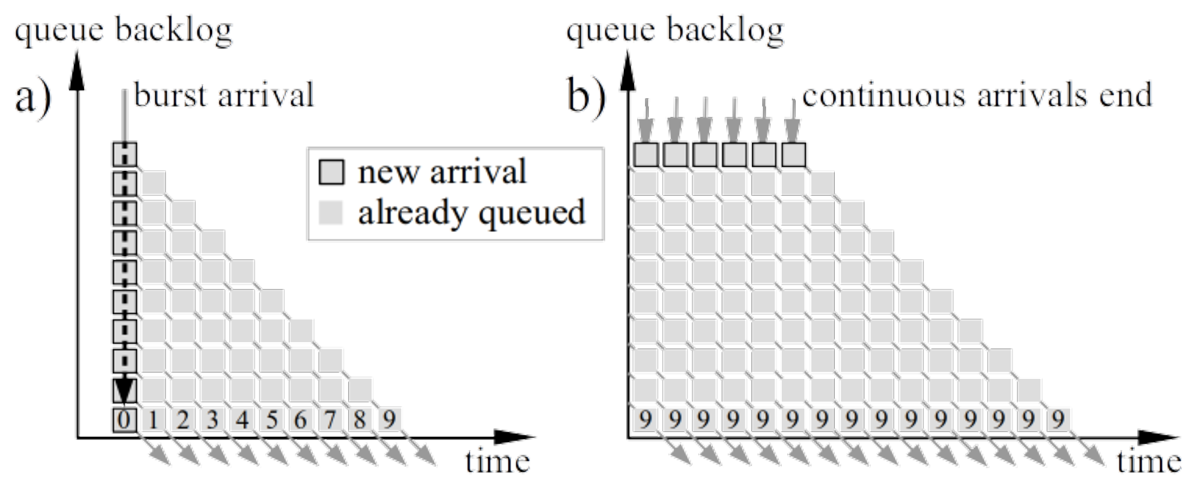
\includegraphics[width=0.8\linewidth]{sojourn-prob}
	\caption{Schematic Illustrating Two Problems with the Sojourn Time Metric. a) It does not measure the full size of a burst until the end (left); b) It does not measure a draining queue (right). Draining is visualized at one equisized packet per timeslot. Sojourn time is represented just before each packet is dequeued as the number of timeslots along its diagonal path.}\label{fig:sojourn-prob}
\end{figure*}

These congestion signals experience delay consisting of the following elements:
\begin{itemize}[nosep]
	\item propagation delay (in common with the data);
	\item queuing delay (in common with the data);
	\item measurement delay: measuring the queue, as well as arrival and/or departure rates;
	\item smoothing delay: filtering out fluctuations in measurements;
	\item signal encoding delay: a number representing the signal is produced within an AQM algorithm, which is then compressed into a unary `encoding' in each packet, and `decoded' by the congestion control algorithm's response to the unary-encoded signals. A unary encoding is used so that the AQM does not have to recognize flows or hold per-flow state. But it constrains the bandwidth of the signalling channel, which introduces encoding delay;
	\item randomization delay: randomness is introduced to break up oscillations, but it requires longer to detect the underlying signal.
\end{itemize}

This memo focuses on reducing two of these: queuing and measurement. The other four are briefly surveyed in \S\,\ref{sec:related}.

The signal from an AQM can be subject to unnecessary queuing delay if it is applied to a packet during the enqueue process, so that it has to work its way through the queue before being transmitted to the line. In classical AQMs, queuing delay is configured to be of the same order of magnitude as typical propagation delays. Therefore subjecting the congestion signal to the delay of the queue will add unnecessary sloppiness to the control loop.

Even if a signal is applied to a packet as it is dequeued, it is often based on a measurement that has taken some time to collect. For instance, the sojourn time technique, which is becoming common for measuring the queue in modern AQMs, gives a queue delay metric that is always out of date by the amount of time the packet spent in the queue. So even if the signal is applied at dequeue, it is delayed by the time spent measuring it in the queue.

The sojourn time measured when a packet reaches the head of the queue takes no account of any change in the queue while that packet is working towards the head. So if a burst (or a reduction in drain rate) extends the queue, the sojourn time of the packet at the front of the burst (or the start of the reduction) will show no evidence of the queue that has built behind it. For instance, on the left of \autoref{fig:sojourn-prob}, the sojourn of the first packet of the burst takes '0' timeslots. And the sojourn time metric only fully measures the burst when the last packet of the burst reaches the head of the queue, where '9' is shown. 

Conversely, consider a queue that has been stable then the flow ends, so that no further packets arrive (the right-hand schematic in \autoref{fig:sojourn-prob}). Then, even when the last packet to arrive is about to be dequeued from the head of the queue, its sojourn time still measures the stable queue delay when it arrived, because that's how long it took to drain the queue. If sojourn alone were used for marking and dropping, there would be no externally visible evidence of the now empty queue behind the last packet until traffic started again.

This memo proposes simple techniques to cut that measurement delay by using all the information available in the queue at the point a packet is dequeued. At the moment a packet is dequeued there is very little time for additional processing, so considerable attention is also paid to minimizing execution time.


